% Intended LaTeX compiler: xelatex
\documentclass[aspectratio=64,12pt]{beamer}
\usepackage{graphicx}
\usepackage{longtable}
\usepackage{wrapfig}
\usepackage{rotating}
\usepackage[normalem]{ulem}
\usepackage{amsmath}
\usepackage{amssymb}
\usepackage{capt-of}
\usepackage{hyperref}
\usepackage{booktabs}
\usepackage{setspace}
\usepackage{quoting}
\usepackage{fancybox}
\institute{Università di Siena}
\usepackage{localheader}
\usepackage{tikz}
\usepackage{booktabs}
\usepackage{setspace}
\usepackage{quoting}
\usepackage[italian]{babel}
\usepackage{fancybox}
\usetheme{default}
\author{Massimo D'Antoni}
\date{Anno accademico 2024-2025}
\title{Lo stato fornitore di beni e servizi\newline (beni pubblici e monopolio)}
\subtitle{Scienza delle Finanze}
\institute{Università di Siena}
\hypersetup{pdfauthor={Massimo D'Antoni},
 pdftitle={Lo stato fornitore di beni e servizi (beni pubblici e monopolio)},
 pdflang={Italian}}
\begin{document}

\maketitle

\section{Definizione di bene pubblico}

%%%%%%%%%%%%%%%%%%%%%%%%%%%%%%%%%%%
\begin{frame}{La nozione di bene pubblico}
I beni pubblici \emph{puri} sono caratterizzati da due proprietà:
\begin{itemize}
\item \alert{non rivalità nel consumo}: una volta fornito il bene ad un individuo, il costo di fornirlo ad un individuo aggiuntivo è nullo;
\item \alert{non escludibilità}: una volta fornito il bene, è impossibile (o molto costoso) escludere qualcuno dal consumo.
\end{itemize}
Conseguenze:
\begin{itemize}
\item la non escludibilità rende impossibile condizionare la fruizione del bene al pagamento di un prezzo;
\item la non rivalità rende inefficiente l'esclusione, anche quando questa è possibile.
\item Nel caso di \emph{fornitura decentrata} o \emph{volontaria} gli individui si comportano da \emph{free-rider}: ciascuno conta sulla fornitura altrui e il livello di bene disponibile risulta inefficientemente basso.
\end{itemize}  
  Nota bene: i beni privati sono \alert{rivali} ed \alert{escludibili} e vi
  sono beni che hanno una sola delle due proprietà.
\end{frame}


%%%%%%%%%%%%%%%%%%%%%%%%%%%%%%%%%%%
\begin{frame}{Esempi}
Sono beni pubblici:
\begin{itemize}
\item la tutela dell'ambiente
\item un'attrazione naturale/paesaggistica
\item il servizio anti-incendi
\item la manutenzione stradale, l'illuminazione stradale, la polizia urbana
\item i servizi di informazione, le trasmissioni televisive (escludibili?)
\item molti beni «immateriali», quali la fiducia reciproca, la condivisione di un linguaggio e di norme comuni
\item \ldots{}o anche un'equa distribuzione del reddito in una società attenta all'equità
\end{itemize}
\emph{Non} sono beni pubblici nel senso indicato:
\begin{itemize}
\item la sanità
\item i trasporti
\end{itemize}
La non rivalità può essere presente in vari gradi.
\end{frame}


%%%%%%%%%%%%%%%%%%%%%%%%%%%%%%%%%%%
\begin{frame}{Precisazioni sulla nozione di bene pubblico}
\begin{itemize}
\item Gli individui consumano il bene pubblico nella stessa quantità, ma il valore che attribuiscono al bene non sarà in generale la stessa per tutti. Da questa differenza nascono molti dei problemi decisionali.
\item Le caratteristiche che rendono pubblico un bene possono cambiare con l'innovazione tecnologica (esempio: escludibilità attraverso sistemi di crittazione dell'informazione)
\item Ci sono beni privati forniti dal pubblico: assistenza sanitaria, servizi di trasporto, istruzione sono escludibili e in buona misura rivali (ma possiamo rintracciare elementi di non rivalità).
\item Ci sono beni pubblici forniti dal privato: assistenza sociale da parte di istituzioni caritative, mecenatismo, e -- su scala ridotta -- gestione di proprietà condominiali.
\item Il concetto di bene pubblico è in parte sovrapposto con quello di esternalità (fornendo un bene pubblico genero un'esternalità positiva per la collettività).
\end{itemize}
\end{frame}


%%%%%%%%%%%%%%%%%%%%%%%%%%%%%%%%%%%
\begin{frame}{Escludibilità/rivalità possono non essere associate}
\begin{center}
\begin{tabular}{lll}
\toprule
 & \emph{rivalità} & \emph{non rivalità}\\[0pt]
\midrule
\emph{escludibilità} & beni privati & beni di club\\[0pt]
\emph{non escludibilità} & risorse comuni (\emph{commons}) & beni pubblici puri\\[0pt]
\bottomrule
\end{tabular}
\end{center}

\begin{itemize}
\item Esempi di beni di club (normalmente presentano un certo grado di rivalità, sono soggetti a congestione): struttura sportiva, piscina, cooperativa di consumo
\begin{itemize}
\item possono essere forniti privatamente dietro pagamento di un prezzo (\emph{membership}); in presenza di rivalità parziale è possibile una fornitura efficiente
\end{itemize}
\item Esempi di risorse comuni: fauna ittica di un lago, risorse naturali
\begin{itemize}
\item può essere visto come un problema di esternalità negativa, il problema è l'eccessivo sfruttamento della risorsa
\end{itemize}
\end{itemize}
\end{frame}

\section{Inefficienza nella fornitura decentrata di beni pubblici}

%%%%%%%%%%%%%%%%%%%%%%%%%%%%%%%%%%%
\begin{frame}{Fornitura volontaria e \emph{free-riding}}
\begin{itemize}
\item Ciascun individuo deve decidere se contribuire (C) o non contribuire (N) alla fornitura di un bene pubblico. Il costo di contribuire è 3.
\item Entrambi gli individui ottengono dal bene pubblico un beneficio 2 se un solo individuo contribuisce, 4 se contribuiscono entrambi. 
\end{itemize}
\vspace{-6pt}
\begin{columns}
\begin{column}{.4\columnwidth}
\begin{center}
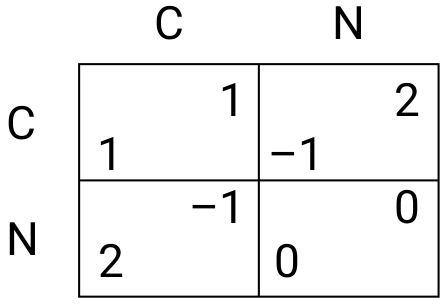
\includegraphics[width=2.5cm]{./figure/gioco-bene-pubblico-dilemma-prigioniero.png}
\end{center}
\vspace{0pt}
\end{column}
\begin{column}{.6\columnwidth}
  Il gioco descrive un \emph{dilemma del prigioniero}: l'equilibrio è NN e il bene non viene fornito.
\end{column}
\end{columns}
\begin{itemize}
\item Un modello alternativo (\emph{weakest link}).  Per avere il bene pubblico è necessario il contributo da parte di \emph{entrambi} gli individui, se uno solo contribuisce non si ha fornitura.
\end{itemize}
\vspace{-6pt}
\begin{columns}
\begin{column}{.4\columnwidth}
\begin{center}
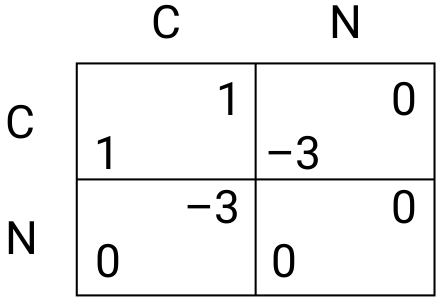
\includegraphics[width=2.5cm]{./figure/gioco-bene-pubblico-coordinamento.png}
\end{center}
\smallskip
\end{column}
\begin{column}{.6\columnwidth}
  Il gioco ha due equilibri di Nash: CC e NN.\\[0pt]
  C'è un problema di coordinamento.\\[0pt]
  Se gli individui si coordinano possono raggiungere l'esito efficiente CC.
\end{column}
\end{columns}
\end{frame}


%%%%%%%%%%%%%%%%%%%%%%%%%%%%%%%%%%%
\begin{frame}{La determinazione del livello efficiente di bene pubblico}
\begin{itemize}
\item Nel caso in cui la scelta non sia semplicemente tra fornire e non fornire, si pone il problema di determinare il \emph{livello efficiente} di un bene pubblico.
\end{itemize}
\begin{columns}
\begin{column}{.3\columnwidth}
\small
\begin{itemize}
\item Il livello di fornitura efficiente può essere individuato in corrispondenza del punto in cui il costo marginale eguaglia la somma dei benefici marginali ($\text{CM}=\sum_{h}\text{BM}^{h}$)
\item sommiamo dunque verticalmente le curve di domanda individuali
\end{itemize}
\end{column}
\begin{column}{.7\columnwidth}
\begin{figure}[htbp]
\centering
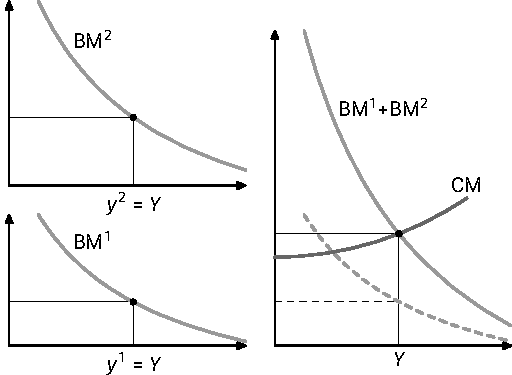
\includegraphics[height=5.5cm]{./figure/domanda-beni-pubblici-2.pdf}
\end{figure} 
\end{column}
\end{columns}
\end{frame}


%%%%%%%%%%%%%%%%%%%%%%%%%%%%%%%%%%%
\begin{frame}{Nel caso del bene privato\ldots{}}
\begin{itemize}
\item Con i beni privati la condizione di efficienza era data dall'eguaglianza tra
costo marginale (offerta) e curva di domanda di mercato, ottenuta come somma
\emph{orizzontale} delle curve di domanda individuali
\begin{equation*}
  \text{BM}^{1}=\text{BM}^{2}=CM
\end{equation*}
\end{itemize}

\begin{center}
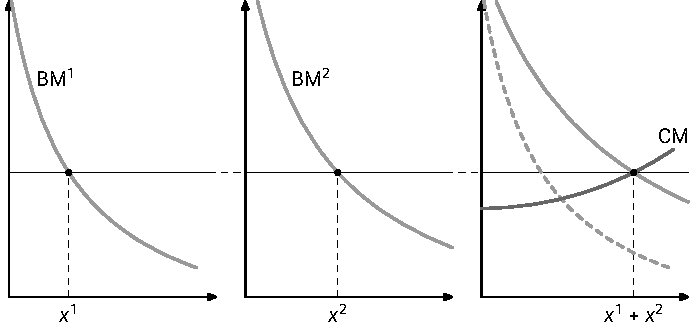
\includegraphics[width=.8\textwidth]{./figure/domanda-beni-pubblici-1.pdf}
\end{center} 
\end{frame}


%%%%%%%%%%%%%%%%%%%%%%%%%%%%%%%%%%%
\begin{frame}{Derivazione della \emph{condizione di Samuelson}}
\begin{columns}
\begin{column}{.5\columnwidth}
\small
\begin{itemize}
\item Una derivazione più rigorosa delle condizioni di efficienza, che dobbiamo a
Samuelson (1954).
\item Efficienza: occorre trovare $x_{1},x_{2},Y$ che realizzano $\max U^{1}$
dato livello $U^{2}$.
\item Occorre ricordare che l'inclinazione della frontiera della possibilità
produttive (FPP) è il SMT.
\item Fissando l'utilità $U^{2}$ tracciamo per differenza verticale la \emph{curva
residuale} (inclinaz. = SMT $-$ SMS$^2$).
\item Nel punto di ottimo E si massimizza l'utilità $U^{1}$ data $U^{2}$ e date
le possibilità produttive.
\end{itemize}
\end{column}

\begin{column}{.5\columnwidth}
\begin{center}
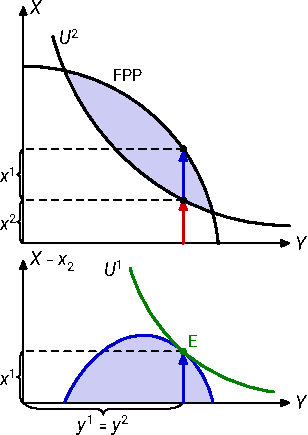
\includegraphics[height=7cm]{./figure/samuelson-11.pdf}\\
La condizione: $\text{SMS}^{1}+\text{SMS}^{2}=\text{SMT}$.
\end{center} 
\end{column}
\end{columns}
\end{frame}


%%%%%%%%%%%%%%%%%%%%%%%%%%%%%%%%%%%
\begin{frame}{Fornitura volontaria e \emph{free riding} nel caso continuo}
\begin{itemize}
\item L'unico equilibrio di Nash del «gioco» di fornitura volontaria del bene
pubblico prevede che l'individuo 1 fornisca la sua quantità preferita
$y^{1}$ e l'individuo 2 non fornisca nulla
\item la quantità fornita $y^{1}$ è \emph{inferiore} alla quantità efficiente $Y^{*}$
\item la conseguente perdita di efficienza è pari all'area ombreggiata
\end{itemize}

\begin{figure}[htbp]
\centering
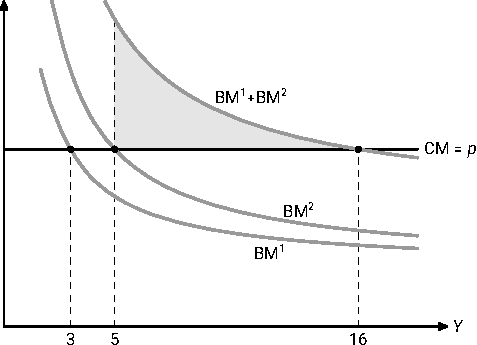
\includegraphics[height=5cm]{./figure/bene-pubblico-equilibrio.pdf}
\end{figure} 
\end{frame}


%%%%%%%%%%%%%%%%%%%%%%%%%%%%%%%%%%%
\begin{frame}{Fornitura volontaria e \emph{free riding} nel caso continuo /2}
\begin{block}{Esercizio}
\small
Con riferimento al grafico della slide precedente, dimostrare che l'\emph{unico}
equilibrio di Nash è quello in cui l'individuo 2 fornisce $y^{2}$ e
l'individuo 1 fornisce zero
\end{block}
\vspace{-2mm}
\small
\begin{itemize}
\item Qual è la quantità fornita da 1 se 2 fornisce zero?
\item Qual è la quantità fornita da 2 in aggiunta a quanto fornito da 1
quando $y^{1}>y^{2}$?
\item Qual è la quantità fornita da 1 se 2 fornisce $y^{2}$? È ancora
ottimale per 2 fornire $y^{2}$ se 1 fornisce una quantità positiva?
\end{itemize}

\begin{block}{Per i pignoli e/o i curiosi}
\footnotesize
\begin{itemize}
\item Ragionando nell'ipotesi che la curva di domanda di ciascuno sia
  indipendente dalla quantità di bene pubblico fornito dagli altri individui
  stiamo escludendo la presenza di effetti di reddito. A parità di bene
  pubblico totale fornito un aumento/riduzione della quantità fornita dagli
  altri comporta infatti un aumento/riduzione del reddito disponibile
  dell'individuo.
\item Come cambierebbe l'analisi volendo tener conto degli effetti di reddito?
\end{itemize}
\end{block}
\end{frame}

%%%%%%%%%%%%%%%%%%%%%%%%%%%%%%%%%%%
\begin{frame}{Applicazione: il sostegno volontario ai poveri}
\begin{itemize}
\item Il sostegno ai poveri quando gli individui sono altruisti può essere visto
come un caso di bene pubblico
\begin{itemize}
  \item Gli individui 1 e 2 sono interessati al benessere dell'individuo 3:
$$U^1(x_1,U^3),\quad U^2(x_2,U^3),\quad U^3(x_3)$$
\item oppure gli individui 1 e 2 sono interessati al fatto che 3 consumi un
  certo bene primario (salute, istruzione)
$$U^1(x_1,x_3),\quad U^2(x_2,x_3),\quad U^3(x_3)$$
\end{itemize}
\item 1 e 2 potranno decidere di finanziare (tramite donazioni) il consumo di 3
\item Ci aspettiamo tuttavia che il consumo di 3 così finanziato sia
inefficientemente basso: utilità e consumo di 3 rappresentano per 1 e 2 un
bene \emph{non rivale} e \emph{non escludibile}. Avremo dunque \emph{free-riding}.
\end{itemize}

\begin{block}{}
Abbiamo descritto l'altruismo come interesse per il benessere altrui.  Una
descrizione alternativa è che gli individui traggano \alert{utilità dall'atto in sé di
donare}.  In questo caso, cosa cambierebbe?
\end{block}
\end{frame}

%%%%%%%%%%%%%%%%%%%%%%%%%%%%%%%%%%%
\begin{frame}{Fornitura di beni non rivali ma escludibili («artificialmente scarsi»)}
\begin{itemize}
\item Se l'esclusione è possibile, sarà possibile condizionare il consumo del bene
al pagamento di un prezzo e quindi finanziare la fornitura del bene
pubblico.  Tuttavia, alcuni individui saranno esclusi dal consumo anche se
il costo (marginale) di un loro accesso al bene è nullo.
\end{itemize}
\begin{figure}[htbp]
\centering
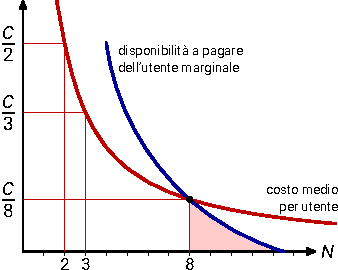
\includegraphics[height=5.5cm]{./figure/beni-pubblici-escludibili-1-color.pdf}
\end{figure}
\end{frame}


%%%%%%%%%%%%%%%%%%%%%%%%%%%%%%%%%%%
\begin{frame}{In sintesi}
Dunque:
\begin{itemize}
\item Senza escludibilità, la soluzione decentrata (volontaria) conduce a un
livello inefficientemente basso -- in alcuni casi nullo -- di bene pubblico
\item Con escludibilità, qualcuno potrà fornire il bene e chiedere un pagamento a
chi vi accede, ma abbiamo comunque una sua sotto-utilizzazione
\end{itemize}
Può un'\alert{autorità pubblica} (ad es. lo Stato) risolvere il problema e garantire la fornitura efficiente del bene pubblico?
\begin{itemize}
\item In astratto ha gli strumenti per farlo: può imporre agli individui di
contribuire al bene anche in assenza di un meccanismo di esclusione (può
utilizzare il proprio potere coercitivo per applicare \alert{imposte});
\item tuttavia l'autorità, anche quando intenzionata ad agire nell'interesse della
collettività, potrebbe non avere l'\alert{informazione} necessaria per individuare
il livello efficiente di bene pubblico, visto che gli individui potrebbero
non avere un incentivo a dichiarare correttamente il beneficio che traggono dal
bene pubblico.
\end{itemize}
\end{frame}


\section{Infrastrutture, servizi di pubblica utilità e monopoli naturali}


%%%%%%%%%%%%%%%%%%%%%%%%%%%%%%%%%%%
\begin{frame}{Infrastrutture e servizi pubblici}
\begin{itemize}
\item Molte infrastrutture/opere pubbliche hanno le caratteristiche di beni
pubblici: ponti, strade, interventi contro il dissesto idrogeologico,
ecc.
\item Altri esempi: la rete di fornitura del servizio idrico, servizi «a rete» che
richiedono rilevanti infrastrutture
\item Anche quando c'è escludibilità e parziale rivalità, la struttura dei
  costi può rendere comunque problematico l'operare di mercati concorrenziali
\item La scala ottimale di produzione è tale da determinare un
  \alert{monopolio naturale}.
\item Il problema di finanziare l'infrastruttura presenta analogie con quello
  già visto di un bene non rivale ed escludibile fornito da privati.
\item Molte infrastrutture sono realizzate dal pubblico, altre sono realizzate in
\emph{project financing}: il governo delega a privati la realizzazione di
un'infrastruttura, che verrà finanziata con i proventi della sua gestione
(fornitura a pagamento agli utenti).
\end{itemize}
\end{frame}

%%%%%%%%%%%%%%%%%%%%%%%%%%%%%%%%%%%
\begin{frame}{Cosa si intende per monopolio naturale}
\begin{itemize}
\item Si ha un monopolio \alert{naturale} quando la concentrazione in un'unica impresa
della produzione per l'intero mercato o per un insieme di mercati risulta
vantaggiosa dal punto di vista dei costi.
\item Nota bene: l'assetto monopolistico dipende dalla struttura dei costi,
  non una disposizione di legge (come sarebbe in un monopolio \alert{legale}).
\item La nozione di monopolio naturale coincide con quella di
\alert{subadditività della funzione di costo}. Se $C(y)$ rappresenta il \alert{minimo}
costo sostenuto da un'impresa per produrre la quantità $y$ (che può essere
un vettore di quantità), abbiamo subadditività dei costi in $y$ se
\begin{gather*}
 C(y) < C(y^1)+C(y^2) \qquad\text{per qualsiasi $y^1,y^2$ tali che $y^1+y^2=y$}\\
 C(y) < C(y^1)+C(y^2)+C(y^3) \qquad\text{per qualsiasi $y^1,y^2,y^3$ tali che $y^1+y^2+y^3=y$}\\
 \text{e così via\dots}
\end{gather*}
\item In presenza di un monopolio naturale \alert{non è efficiente} avere più di un'impresa
sul mercato, e ci aspettiamo che il mercato tenda naturalmente al \alert{monopolio}.
\end{itemize}
\end{frame}

%%%%%%%%%%%%%%%%%%%%%%%%%%%%%%%%%%%
\begin{frame}{Economie di scala}
\begin{itemize}
\item \alert{Definizione}: il costo di produzione aumenta meno che
proporzionalmente rispetto alla quantità prodotta, ovvero:
\begin{equation*}
 C(ky) < kC(y) \qquad\text{se }k>1
\end{equation*}
\item ciò equivale alla condizioni di \alert{costi medi decrescenti}
\begin{equation*}
\frac{C(ky)}{ky} < \frac{kC(y)}{ky} = \frac{C(y)}{y} 
\end{equation*}
\item se il costo medio è decrescente, \alert{il costo marginale è inferiore al costo
medio} (sapreste dimostrarlo formalmente?)
\item La presenza di economie di scala
implica la subadditività della funzione di costo.
\end{itemize}
\end{frame}


%%%%%%%%%%%%%%%%%%%%%%%%%%%%%%%%%%%
\begin{frame}{Un semplice esempio di economie di scala}
\begin{itemize}
\item Una caso semplice: costi variabili/marginali costanti in presenza di costi fissi.
\begin{itemize}
\item Costo totale: $C(y)=F+cy$
\item Costo medio: $CM(y)=c+F/y$
\item Costo marginale: $c$
\end{itemize}
\end{itemize}
\begin{figure}[htbp]
\centering
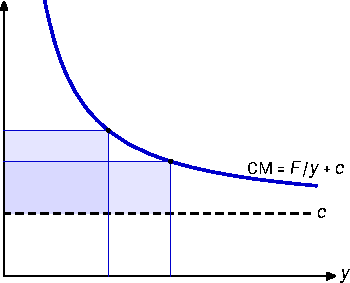
\includegraphics[height=5cm]{./figure/monopolio-naturale-1-color.pdf}
\end{figure}
\end{frame}


%%%%%%%%%%%%%%%%%%%%%%%%%%%%%%%%%%%
\begin{frame}{L'impresa multiprodotto}
\begin{itemize}
\item La definizione di monopolio naturale si può estendere al caso di imprese
multiprodotto. In questo caso occorre considerare come variano i costi nel
caso di produzione congiunta di più beni.
\item \alert{Economie di diversificazione}: conviene produrre due beni congiuntamente
invece che separatamente (es. condivisione di costi fissi). Formalmente:
\begin{equation*}
 C(y_1,y_2)=F + c_1y_1+c_2y_2 \qquad C(y_1)=F + c_1y_1 \qquad  C(y_2)=F + c_2y_2 
\end{equation*}
\item Quando posso utilizzare infrastrutture o funzioni comuni per operare in diversi mercati
\begin{itemize}
\item Esempio: un servizio postale che utilizza la propria rete di sportelli per
fornire anche servizi bancari.
\end{itemize}
\item La presenza di economie di scala e di economie di diversificazione implica
la subadditività della funzione di costo nel caso multiprodotto.
\end{itemize}
\end{frame}

%%%%%%%%%%%%%%%%%%%%%%%%%%%%%%%%%%%
\begin{frame}{Quali sono le conseguenze di un monopolio naturale?}
\begin{itemize}
\item È inefficiente (e spesso non attuabile) forzare la concorrenza in un contesto
caratterizzato da economie di scala ed economie di diversificazione.
\item Per evitare che il monopolista (privato) spinto dalla ricerca del profitto
scelga un prezzo inefficientemente alto, è possibile:
\begin{itemize}
\item \alert{regolamentare} il monopolio privato;
\item \alert{nazionalizzare} il settore e creare un monopolio pubblico.
\end{itemize}

\item Di seguito ci occuperemo di come regolamentare un monopolista privato, ma
l'analisi si applica, con poche differenze, al problema di fissare le
tariffe nel caso di un monopolio pubblico
\end{itemize}
\end{frame}

%%%%%%%%%%%%%%%%%%%%%%%%%%%%%%%%%%%
\begin{frame}{La scelta del monopolista che massimizza i profitti}
\begin{columns}
\begin{column}{.45\columnwidth}
\begin{itemize}
\item Massimizzazione del profitto:
\begin{equation*}
\max_{p}\; py(p)-[F+cy(p)]
\end{equation*}
\item condizioni del I ordine:
\begin{equation*}
y(p) + py'(p) - cy'(p)=0
\end{equation*}
\item il prezzo scelto dal monopolista sarà
\begin{equation*}
\frac{p-c}{p}=\frac{-y(p)}{py'(p)}=\frac{1}{\epsilon}
\end{equation*}
dove $\epsilon>1$ è l'elasticità della domanda.
\item Il prezzo è superiore al costo medio (e quindi al
costo marginale)
\end{itemize}
\end{column}

\begin{column}{.55\columnwidth}
\begin{figure}[htbp]
\centering
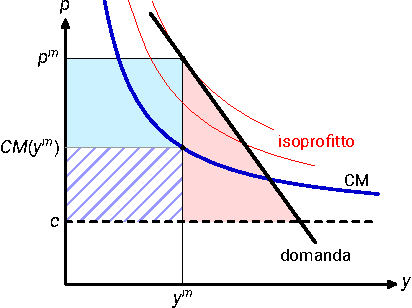
\includegraphics[height=5cm]{./figure/monopolio-naturale-2-color.pdf}
\end{figure}

\begin{itemize}
\item Nel grafico: l'area azzurra è il profitto, l'area rossa è la perdita di benessere (inefficienza), il costo fisso corrisponde all'area tratteggiata
\end{itemize}
\end{column}
\end{columns}
\end{frame}


%%%%%%%%%%%%%%%%%%%%%%%%%%%%%%%%%%%
\begin{frame}{Perché l'esercizio di potere monopolistico è inefficiente?}
\begin{itemize}
\item \alert{Inefficienza allocativa} (prezzo > costo marginale): alcuni
  consumatori non accedono al bene/servizio sebbene tale accesso comporti
  benefici che eccedono i costi.
\item \alert{Inefficienza-X} (o manageriale): il monopolista ha scarso incentivo a
contenere i costi. J. Hicks: «The best of all economic rents is quiet life»
\end{itemize}

Rispetto al primo problema, l'autorità pubblica può \alert{regolare il prezzo}, fissandolo a un livello inferiore al prezzo di monopolio.
\begin{itemize}
\item Prezzo pari al \alert{costo medio}: garantisce la copertura dei costi e nessun
extra-profitto
\item Prezzo pari al \alert{costo marginale}: impone al monopolista una perdita
\end{itemize}
\begin{block}{}
  \small
\begin{itemize}
\item Nella definizione di costo della microeconomia è compreso il \alert{costo del
capitale}: interessi ma anche quella parte di profitti necessaria a remunerare
il capitale di rischio (profitto «normale»)
\item Quando si parla di profitto, si intende extra-profitto (rendita monopolistica)
\end{itemize}
\end{block}
\end{frame}


%%%%%%%%%%%%%%%%%%%%%%%%%%%%%%%%%%%
\begin{frame}{È proprio necessario regolamentare un monopolio naturale?}
\begin{itemize}
\item Demsetz (1967) mise in dubbio che le economie di scala fossero condizione
\alert{sufficiente} per regolare il mercato;
\item la concorrenza \alert{nel} mercato è resa impossibile dalla presenza di
economie di scala, ma può esserci concorrenza \alert{per il} mercato;
\item azione disciplinante della minaccia di entrata da parte di nuovi operatori: se il monopolista ottiene (extra)profitti positivi, spingerà altre imprese a
entrare nel mercato, offrendo prezzi più bassi;
\item si parla di \alert{mercato contendibile}.
\end{itemize}
\begin{block}{}
  \small
  La \alert{teoria del mercati contendibili}, popolare a fine anni
  '70 e negli anni '80:
  
- condizione cruciale è che il monopolista non sia in grado di reagire
  all'entrata di un concorrente con sufficiente rapidità;

- assumono rilevanza i costi «affondati» (\emph{sunk costs}): l'entrata avverrà
solo se possibile una concorrenza \emph{hit \& run} in cui a seguito della
reazione del monopolista l'entrante può uscire senza costi;

- queste condizioni si verificano molto raramente.

\end{block}
\end{frame}

%%%%%%%%%%%%%%%%%%%%%%%%%%%%%%%%%%%
\begin{frame}{Politiche tariffarie per un monopolio regolamentato: costo medio}
\begin{itemize}
\item Il minor prezzo compatibile con l'assenza di perdite è $p=c+F/y$ (\alert{costo medio}),
che tuttavia non elimina del tutto l'inefficienza allocativa
\end{itemize}

\begin{figure}[htbp]
\centering
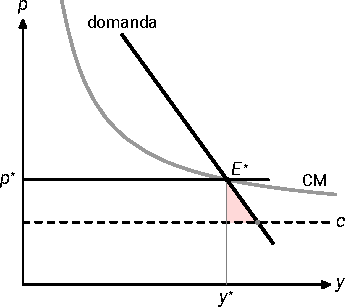
\includegraphics[height=6cm]{./figure/monopolio-naturale-4-color.pdf}
\end{figure}
\end{frame}


%%%%%%%%%%%%%%%%%%%%%%%%%%%%%%%%%%%
\begin{frame}{Politiche tariffarie per un monopolio regolamentato: costo marginale}
\begin{itemize}
\item Il prezzo ottimale dal punto di vista allocativo è pari al \alert{costo marginale}
$p=c$, ma in presenza di economie di scala tale prezzo rende impossibile la
copertura dei costi fissi $F$: è necessario coprire i costi fissi con un sussidio.
\end{itemize}

\begin{figure}[htbp]
\centering
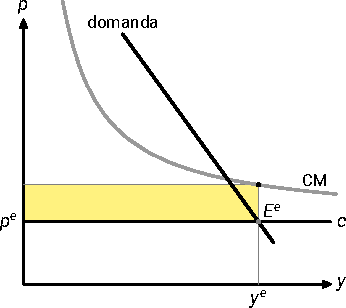
\includegraphics[height=5cm]{./figure/monopolio-naturale-3-color.pdf}
\end{figure}

\begin{itemize}
\item Perché prevedere un sussidio potrebbe essere un problema?
\end{itemize}
\end{frame}


%%%%%%%%%%%%%%%%%%%%%%%%%%%%%%%%%%%
\begin{frame}{Politiche tariffarie: tariffa in due parti, menu di tariffe\ldots{}}
\begin{itemize}
\item In alcuni casi è possibile coprire il costo fisso adottando una
\alert{tariffa in due parti}. Il prezzo complessivo pagato dal consumatore/utente
risulta $E^i(p)=E+py^i$ (canone $E$)
\begin{itemize}
\item Se $E=F/N$ ($N$ = numero utenze) copriamo interamente i costi fissi.
\item È una soluzione in gradi di eliminare l'inefficienza allocativa? In
generale no, visto che il canone potrebbe scoraggiare gli utenti con bassa
domanda, spingendoli ad astenersi dal consumo.
\end{itemize}
\item Spesso l'offerta prevede un \alert{menu di tariffe in due parti}:
\begin{itemize}
\item Non potendo discriminare tra utenti ad alta/bassa domanda, li spingiamo a
scegliere la tariffa più coerente con il loro livello di domanda: gli
utenti a bassa domanda scelgono prezzo più alto e canone basso o nullo,
gli utenti a domanda più elevata scelgono canone più elevato e prezzo più
basso (al limite pari al costo marginale)
\item Esempio: 0,15€ con scatto alla risposta oppure tariffa «flat» di 5€/mese
senza scatto alla risposta
\end{itemize}
\end{itemize}
\end{frame}


%%%%%%%%%%%%%%%%%%%%%%%%%%%%%%%%%%%
\begin{frame}{Il monopolista multiprodotto (o multimercato)}
\begin{itemize}
\item Se deve essere garantito il pareggio di bilancio, in assenza di canone,
  il vincolo di bilancio di un monopolista che opera su due mercati è:
\begin{equation*}
 p_1y_1+p_2y_2=F+c_1y_1+c_2y_2
\end{equation*}
ovvero:
\begin{equation*}
 (p_1-c)y_1+(p_2-c)y_2=F
\end{equation*}
\begin{itemize}
\item Qual è il modo ottimale di imputare il costo fisso $F$ ai due prodotti?
\item Esiste un criterio ispirato all'efficienza?
\end{itemize}
\item Un problema simile si presente quando il monopolista, pur producendo un
prodotto omogeneo, può \alert{discriminare} il prezzo tra diverse categorie di
utenti, segmentando il mercato (in base all'età o altre caratteristiche,
utenza domestica/d'affari, ecc.)
\begin{itemize}
\item È desiderabile tale discriminazione?
\end{itemize}
\end{itemize}
\end{frame}

%%%%%%%%%%%%%%%%%%%%%%%%%%%%%%%%%%%
\begin{frame}{Tariffazione efficiente del monopolista multiprodotto}
\begin{figure}[htbp]
\centering
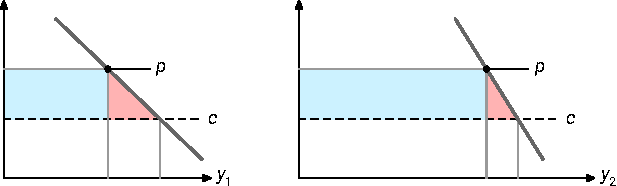
\includegraphics[width=.7\textwidth]{./figure/ramsey-1-color.pdf}
\end{figure}

A parità di gettito complessivo (le due aree azzurre), al fine di ridurre la perdita
di benessere (le due aree rosse) conviene abbassare il prezzo nel primo mercato (dove
la domanda è più elastica) e alzarlo nel secondo (dove la domanda è più
rigida)

\begin{figure}[htbp]
\centering
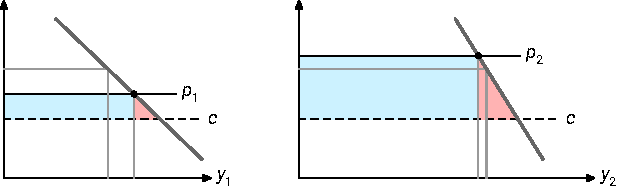
\includegraphics[width=.7\textwidth]{./figure/ramsey-2-color.pdf}
\end{figure}
\end{frame}


%%%%%%%%%%%%%%%%%%%%%%%%%%%%%%%%%%%
\begin{frame}{La regola dell'elasticità inversa}
\begin{figure}[htbp]
\centering
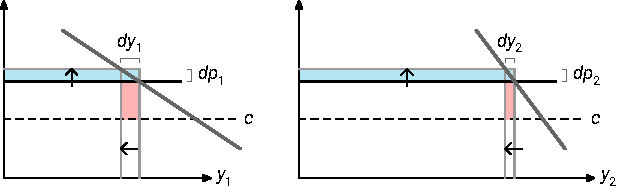
\includegraphics[height=3.6cm]{./figure/ramsey-3-color.pdf}
\end{figure}

\begin{itemize}
\item La medesima variazione del prezzo determina nei due mercati una diversa variazione dei ricavi e
della perdita di benessere.
\item Se le domande dei due beni sono indipendenti (il prezzo dell'uno non influenza la domanda dell'altro), l'ottimo è identificato dalla regola dell'elasticità inversa:
\begin{equation*}
\frac{(p_1-c)/p_1}{(p_2-c)/p_2}=\frac{\epsilon_2}{\epsilon_1}
\end{equation*}
\end{itemize}
\end{frame}

%%%%%%%%%%%%%%%%%%%%%%%%%%%%%%%%%%%
\begin{frame}{Le regola dell'elasticità inversa /2}
\begin{columns}
\begin{column}{.57\columnwidth}
\begin{itemize}
\item Nell'ottimo deve essere uguale, per tutti i mercati, il rapporto tra l'effetto marginale di un aumento del prezzo sulla perdita di benessere e l'effetto marginale dello stesso aumento sui ricavi:
\begin{equation*}
  \lambda_i=
  \frac{\textcolor{red!30!white}{\rule{3mm}{3mm}}}{\textcolor{cyan!30!white}{\rule{3mm}{3mm}}-
        \textcolor{red!30!white}{\rule{3mm}{3mm}}}=
  \frac{(-dy_i)(p_i-c)}{dp_iy_i-(-dy_i)(p_i-c)}
\end{equation*}
\item fissando $\lambda_i=\lambda$ (uguale per tutti i mercati):
\begin{equation*}
   \frac{p_i-c}{p_i} = -\frac{\lambda}{1+\lambda}\frac{y_idp_i}{p_idy_i} = \frac{\lambda}{1+\lambda}\frac{1}{\varepsilon_i} 
\end{equation*}
\end{itemize}
\end{column}

\begin{column}{.43\columnwidth}
\begin{figure}[htbp]
\centering
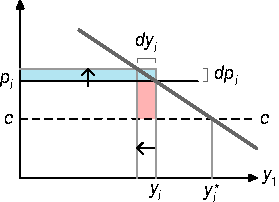
\includegraphics[height=4cm]{./figure/ramsey-4-color.pdf}
\end{figure}
\end{column}
\end{columns}

\medskip
\begin{itemize}
\item La generalizzazione di questa regola al caso in cui le domande non sono
indipendenti, per cui occorre tenere conto anche degli effetti «incrociati» tra diversi prezzi, è nota come \alert{regola di Ramsey} (si parla di prezzi o tariffe \emph{à la} Ramsey)
\end{itemize}
\end{frame}


%%%%%%%%%%%%%%%%%%%%%%%%%%%%%%%%%%%
\begin{frame}{Discriminazione, efficienza ed equità delle politiche tariffarie}
\begin{itemize}
\item L'analisi svolta indica che in generale è efficiente consentire la
discriminazione degli utenti mediante tariffe differenziate, menu di tariffe
ecc.
\item Osserviamo che la discriminazione corrisponde alla strategia ottimale anche
per un monopolista che vuole massimizzare i profitti.
\begin{itemize}
\item La differenza è nel \alert{livello} delle tariffe, che il regolatore
  fissa al minimo compatibile con la copertura dei costi, mentre il
  monopolista fisserebbe a un livello più alto, in modo da massimizzare i profitti.
\end{itemize}
\item Quando diciamo \alert{ottimale} intendiamo \alert{efficiente}
\begin{itemize}
\item Passando da una tariffa uniforme a una tariffa differenziata avremo in
molti casi vincitori e perdenti. Il punto è che il guadagno per chi vince
è maggiore della perdita per chi perde
\end{itemize}
\item Se guardiamo all'equità\ldots{}
\begin{itemize}
\item Con la regola dell'elasticità inversa abbiamo prezzi più alti dove la domanda è più rigida. Gli utenti a domanda rigida potrebbero essere meno abbienti
\end{itemize}
\end{itemize}
\end{frame}

\section{Informazione, incentivi e assetto proprietario}


%%%%%%%%%%%%%%%%%%%%%%%%%%%%%%%%%%%
\begin{frame}{L'informazione del regolatore}
\begin{itemize}
\item L'applicazione delle tariffe ottimali richiede la conoscenza delle
condizioni di domanda e i costi sostenuti dalle imprese regolamentate.
\item Possiamo pensare alle relazione tra regolatore e impresa regolata come a un
caso di relazione \alert{principale/agente}, nella quale un certo compito (fornire
il servizio) è delegato dal principale (la collettività, tramite lo Stato)
all'agente (l'impresa), ma quest'ultimo gode di un vantaggio informativo.
\item Nota bene:
\begin{itemize}
\item al regolatore/principale non basta conoscere il costo effettivamente
  sostenuto, occorre sapere se tale costo sia effettivamente il \alert{minimo
    costo};
\item non c'è differenza tra regolare il prezzo di vendita di beni e servizi agli utenti
(es. servizio idrico, trasporti) e fissare il prezzo per la fornitura diretta di beni allo Stato
(\emph{procurement} in campo medico, militare, realizzazione di infrastrutture) o
per lo svolgimento di servizi (es. riscossione tributi).
\end{itemize}
\end{itemize}
\end{frame}

%%%%%%%%%%%%%%%%%%%%%%%%%%%%%%%%%%%
\begin{frame}{Una soluzione: l'asta}
\begin{itemize}
\item Realizza in effetti la concorrenza «per il» mercato.
\item È anche un modo per limitare/eliminare lo svantaggio informativo del «principale»:
\begin{itemize}
\item se i partecipanti hanno costi simili, il prezzo dichiarato nell'offerta
  dovrà essere vicino al minimo costo medio.
\end{itemize}
\item Il ricorso all'asta non è tuttavia privo di controindicazioni o limiti:
\begin{itemize}
\item potrebbero esserci pochi partecipanti all'asta;
\item i partecipanti potrebbero colludere.
\end{itemize}
\item Inoltre, l'asta definisce le condizioni di fornitura del servizio, ma tali
condizioni possono mutare nel tempo:
\begin{itemize}
\item al rinnovo dell'asta, non c'è simmetria tra i partecipanti, il
  monopolista può godere di un vantaggio rispetto ai competitori, specie se
  l'asta è infrequente;
\item d'altra parte, aste troppo frequenti possono indurre il monopolista ad
  adottare un'ottica di breve periodo;
\item come regolarsi per gli investimenti a lungo termine?
\end{itemize}
\end{itemize}
\end{frame}

%%%%%%%%%%%%%%%%%%%%%%%%%%%%%%%%%%%
\begin{frame}{Incentivi e rendite}
\begin{itemize}
\item La presenza di informazione asimmetrica può determinare, a seconda della
soluzione adottata, una \alert{diluizione degli incentivi} o la creazione di
\alert{rendite} in capo al monopolio regolamentato.
\item Un semplice modellino:
\begin{itemize}
\item ipotizziamo che il regolatore possa osservare il costo di produzione $C$, ma
non sappia se un costo elevato è dovuto a condizioni esogene avverse o a
inefficienza dell'impresa: $C=\theta-e$, dove $\theta$ può essere alto
o basso ($\theta_a>\theta_b$);
\item ridurre $e$ è costoso, il livello ottimale $e^*$ sarà realizzato solo se
ci sono incentivi appropriati a farlo;
\item all'impresa deve essere garantita la copertura dei costi, altrimenti il
servizio non sarà fornito.
\end{itemize}
\item Consideriamo due possibili «contratti» regolatori, le due
soluzioni estreme al problema dell'asimmetria informativa e degli incentivi:
\begin{itemize}
\item \emph{fix price}: prezzo predeterminato che prescinde dal valore
  osservato di $C$.
\item \emph{cost plus}: prezzo fissato in modo da coprire i costi sostenuti e osservati $C$.
\end{itemize}
\end{itemize}
\end{frame}

%%%%%%%%%%%%%%%%%%%%%%%%%%%%%%%%%%%
\begin{frame}{Schemi regolatori \emph{fix-price} e \emph{cost-plus}}
\begin{itemize}
\item Con il \emph{fix-price} scelgo un prezzo $\bar P$, da applicare a
prescindere dal valore osservato di $C$:
\begin{itemize}
\item il monopolista percepisce un profitto $\bar P - C = \bar P - \theta +
    e$. Visto che un aumento di $e$ si traduce in maggiori profitti, sceglierà
$e^*$;
\item il prezzo dovrà garantire un profitto non negativo, dunque $\bar P=\theta_a-e^*$;
\item quando il costo esogeno è $\theta_b$ (inferiore a $\theta_a$), il
monopolista percepisce un extra-profitto $\bar P-\theta_b+e^*=\theta_a-\theta_b>0$.
\end{itemize}
\item Con il \emph{cost-plus} scelgo un prezzo sempre pari al costo osservato $C$:    
\begin{itemize}
\item il monopolista percepisce un profitto $P-C=0$ a prescindere dalla scelta
di $e$, dunque sceglierà il minimo valore di $e$ (mettiamo che sia $e=0$);
\item il prezzo risulterà dunque essere $P=\theta_a$ oppure $P=\theta_b$
\end{itemize}
\item Attribuendo una probabilità $\pi$ al caso $\theta_a$ e $1-\pi$ al caso
$\theta_b$, la soluzione \emph{fix-price} risulterà conveniente se e solo se
\begin{equation*}
   \underbrace{\bar P=\theta_a-e^*}_{\text{prezzo atteso fix-price}}
   <\quad\underbrace{\pi\theta_a+(1-\pi)\theta_b.}_{\text{prezzo atteso cost-plus}}
\end{equation*}
\end{itemize}
\end{frame}

%%%%%%%%%%%%%%%%%%%%%%%%%%%%%%%%%%%
\begin{frame}{Schemi regolatori \emph{fix-price} e \emph{cost-plus} /2}
\begin{itemize}
\item Dalla formula precedente ricaviamo che la soluzione \emph{fix-price} risulta
conveniente se e solo se
\begin{equation*}
   (1-\pi)(\theta_a-\theta_b)<e^*.
\end{equation*}
cioè se il valore atteso della rendita è superiore al risparmio $e^*$ nei
costi determinato dall'incentivo a produrre in modo efficiente.
\item La scelta della soluzione \emph{fix-price} risulterà dunque tanto più
conveniente
\begin{itemize}
\item quanto più è probabile che il costo sia alto ($\pi$ alto);
\item quanto minore è l'impatto della componente esogena del costo ($\theta_a-\theta_b$);
\item quanto maggiore è la riduzione nei costi $e^*$ determinata dall'incentivo;
\item quanto meno problematico è che il monopolista consegua
una rendita.
\end{itemize}
\item Vi saranno casi nei quali è preferibile la soluzione meno incentivante rappresentata dal \emph{cost-plus}
\item Una soluzione intermedia tra \emph{fix-price} e
\emph{cost-plus} può trovare l'ottimo compromesso tra incentivi e riduzione della
rendita del monopolista.
\end{itemize}
\end{frame}

%%%%%%%%%%%%%%%%%%%%%%%%%%%%%%%%%%%
\begin{frame}{La «regolazione incentivante»}
\begin{itemize}
\item \emph{Regolazione tradizionale}
\begin{itemize}
\item auditing periodico dei costi
\item adeguamento «continuo» dei prezzi alla struttura dei costi
\item i guadagni di efficienza passano immediatamente ai consumatori
\item garanzia di un adeguato tasso di profitto al monopolista
\item incentivo ad investire (aumentano i profitti riconosciuti), temperato da
valutazione da parte del regolatore
\end{itemize}
\item \emph{Regolazione incentivante}
\begin{itemize}
\item tetti predeterminati ai prezzi (\emph{price cap})
\item adozione di formula «rigida» di adeguamento dei prezzi, con allineamento
ogni $n$ anni
\item aumenti di efficienza si traducono in profitti per l'impresa (che possono
essere maggiori o minori del profitto «normale»)
\item incentivo ad investire per aumentare l'efficienza, ma spesso prevale
un'ottica di breve periodo (vedi riallineamento periodico, rinnovo
concessione\ldots{})
\end{itemize}
\item È evidente l'analogia tra regolazione incentivante e schemi \emph{fix-price}.
\end{itemize}
\end{frame}

\section{Fornitura pubblica o privata?}


%%%%%%%%%%%%%%%%%%%%%%%%%%%%%%%%%%%
\begin{frame}{Regolazione o fornitura pubblica?}
\begin{itemize}
\item La responsabilità pubblica di fornire un servizio efficiente non richiede
necessariamente la fornitura diretta pubblica
\begin{itemize}
\item Alcuni servizi sono forniti dal pubblico (es. difesa, ordine pubblico,
amministrazione della giustizia\ldots{}), per altri si prevede la delega a un
fornitore privato (es. trasporti e altri servizi di pubblica utilità)
\item \alert{Privatizzazione}: passaggio dal pubblico al privato, ma può voler dire
molte cose (mutamento della forma giuridica, cessione del controllo
parziale o totale)
\end{itemize}
\item A partire dagli anni '80 e '90 tendenza alla privatizzazione di molti
servizi nei paesi dell'Europa occidentale. Le ragioni:
\begin{itemize}
\item cambiamenti tecnologici (minore incidenza delle economia di scala);
\item ragioni «ideologiche»: maggiore attenzione all'efficienza rispetto agli
  obiettivi di garanzia di accesso universale e finalità redistributive;
  l'emergere di un orientamento pro-mercato e favorevole alle soluzioni
  di mercato;
\item pressioni di bilancio, spinta a «fare cassa» tramite vendita di proprietà
pubblica.
\end{itemize}
\end{itemize}
\end{frame}


%%%%%%%%%%%%%%%%%%%%%%%%%%%%%%%%%%%
\begin{frame}{Regolazione o fornitura pubblica? /2}
Ci sono ragioni per preferire una soluzione o l'altra?
\begin{itemize}
\item La privatizzazione appare in molti casi una precondizione per una maggiore
apertura alla concorrenza
\begin{itemize}
\item i processi di privatizzazione si sono accompagnati alla liberalizzazione
di alcuni segmenti di mercato, dis-integrazione verticale rispetto alla
precedente struttura verticalmente integrata
\end{itemize}
\item «Il privato è più efficiente». Vale anche quando l'impresa privata opera in
condizioni di monopolio?
\begin{itemize}
\item La motivazione del profitto spinge gli azionisti a monitorare maggiormente
l'operato del management.
\item Il «mercato della proprietà» e il rischio di scalata ostile o di
fallimento rappresentano fattori di disciplina. L'impresa pubblica è
soggetta a un \emph{soft budget constraint}.
\end{itemize}
\item Le analisi empiriche mostrano spesso una maggiore efficienza (costi
inferiori) delle imprese private, ma difficile stabilire il rapporto
causa-effetto
\end{itemize}
\end{frame}

%%%%%%%%%%%%%%%%%%%%%%%%%%%%%%%%%%%
\begin{frame}{A favore della produzione pubblica}
\begin{itemize}
\item Non tutte le attività sono «privatizzabili». Ma dove collochiamo il confine?
\item In astratto, possiamo spingere l'impresa orientata al profitto ad agire
nell'interesse collettivo specificando in modo dettagliato i termini e la
«qualità» del servizio desiderato.
\item Nella realtà, tale specificazione è difficile, il «contratto» tra regolatore
e regolato è necessariamento \emph{incompleto}
\item L'\alert{incompletezza contrattuale} può rendere in molti casi la soluzione
pubblica preferibile, quando alcune dimensioni del servizio non sono ben
specificabili in anticipo e la rinegoziazione del contratto non appare una
soluzione adeguata
\begin{itemize}
\item Si paga un prezzo in termini di efficienza produttiva (costi), visto che
l'indeterminatezza degli obiettivi si traduce in un \emph{soft budget
constraint}.
\end{itemize}
\end{itemize}
\end{frame}

%%%%%%%%%%%%%%%%%%%%%%%%%%%%%%%%%%%
\begin{frame}{Esempio: la privatizzazione delle prigioni}
\begin{itemize}
\item Hart-Shleifer-Vishny (1997) considerano il caso delle prigioni americane:
\begin{itemize}
\item obiettivo multidimensionale («qualità» che comprende il rispetto dei
diritti umani dei carcerati) non definibile in un contratto;
\item l'applicazione di incentivi troppo forti al risparmio spinge a
privilegiare le dimensioni «verificabili» rispetto a quelle «non
verificabili» (un problema generale di ogni schama di incentivi);
\item vi sono casi in cui è meglio rinunciare a minimizzare i costi se non si è
sicuri che questo non comprometta altri obiettivi rilevanti.
\end{itemize}
\item La produzione pubblica (no delega ai privati) garantisce in molti casi un
migliore bilanciamento quando alcuni degli obiettivi non sono «verificabili»
e quindi non sono contrattabili con sufficiente precisione
\end{itemize}
\end{frame}

%%%%%%%%%%%%%%%%%%%%%%%%%%%%%%%%%%%
\begin{frame}{Le \emph{authority} di settore}

\begin{itemize}
\item Per limitare le occasioni di intervento discrezionale dello Stato
  (o ente locale) sono state spesso istituite delle autorità
  (\emph{authority}) settoriali. In Italia:
\begin{itemize}
\item A. per l'energia elettrica e il gas (1995), poi A. di Regolazione
  per Energia Reti e Ambiente, ARERA;
\item A. per le garanzie nelle telecomunicazioni, AGCOM (1997);
\item A. di regolazione dei trasporti (2011);
\end{itemize}
\item Le autorità operano in modo autonomo nell'interesse pubblico, con un
  mandato molto più definito rispetto alle istituzioni di governo nazionale e
  territoriale.
\end{itemize}
\end{frame}
\end{document}
